\documentclass[a4paper, twocolumn, superscriptaddress, longbibliography]{revtex4-2}
\usepackage[colorlinks,urlcolor=blue,linkcolor=blue]{hyperref}
\usepackage[utf8]{inputenc}
\usepackage{graphicx}
\usepackage{geometry}
\usepackage{amsmath}
\usepackage{amssymb}
\usepackage{amsfonts}
\usepackage{hyperref}
\usepackage{dsfont}
\usepackage[dvipsnames]{xcolor}
\usepackage{appendix}

\hypersetup{citecolor=cyan}
\geometry{hmargin=2cm,vmargin=2cm}

\begin{document}
	\author{Maxime Debertolis}
	%\email{maxime.debertolis@uni-bonn.de}
	\affiliation{Institute of Physics, University of Bonn, Nu\ss allee 12, 53115 Bonn, Germany}
	\title{Gaussian augmented Tensor Networks for universal quantum simulations}

	\begin{abstract}

	\end{abstract}

	\maketitle

	\emph{Introduction}: Adaptation of the stabilizer tensor network formalism developed in~\cite{Masot_Llima_2024} for Gaussian operations instead of stabilizer ones. \\
	
	Ansatz mixing a basis of orbitals to an MPS:
	\begin{equation}
		|\psi \rangle = \sum_{i=1}^{2^{L}} \nu_i^{} d_{\vec{b}_i}^{} |\psi_{\mathrm{G}}^{}\rangle,
	\end{equation}
	\emph{Gaussian states}:
	Majorana operators and fermionic operators are related as:
	\begin{equation}
		\gamma_{2j-1} = c^{\dagger}_{j} + c_{j}, \;\;
		\gamma_{2j} = -i ( c^{\dagger}_{j} + c_{j}),
	\end{equation}
	Covariance matrix: 
	\begin{equation}
		\Gamma_{ab}^{} = \frac{i}{2} \mathrm{Tr}\left(\rho[\gamma_a^{},\gamma_b^{}] \right)
	\end{equation}
	Diagonalizing the matrix $\Gamma$ corresponds to a rotation of the majorana modes by a $2L\times2L$ matrix $R$, which we dub the \emph{stabilized basis} and denoted in the following by a single tilda on the operators:
	\begin{equation}
		\tilde{\gamma}_j = \sum_{k=1}^{2L} R_{jk}\gamma_{k}
	\end{equation}
	The state can be simply written using the majorana modes or the corresponding orbitals if it is pure:
	\begin{equation}
		\begin{split}
			|\psi_{\mathrm{G}}\rangle &= \prod_{j=1}^{L}\left(\tilde{c}_{j}^{\dagger}\right)^{n_j}|0\rangle, \\
			\rho_{\mathrm{G}}^{} &= \frac{1}{2^{L}}\prod\limits_{j=1}^{2L}\left(\mathds{1} + i\lambda_{j} \tilde{\gamma}_{2j-1}^{} \tilde{\gamma}_{2j}^{} \right)
		\end{split}
	\end{equation}
	This is valid in a given basis, where $n_j=\langle c^{\dagger}_j c^{}_j\rangle=(1+\lambda_j)/2$ are the occupations of orbital $j$, and are known from the diagonalization of the covariance matrix. From this set of rotated operators, we can define a set of $L$ \emph{stabilizers}, which together completely determine the stabilized state:
	\begin{equation}
		S_{i} = 
		\begin{cases}
			\tilde{n}_i \quad &\text{if} \quad \langle \tilde{n}_i \rangle = 1 \\
			1 - \tilde{n}_i \quad &\text{if} \quad \langle \tilde{n}_i \rangle = 0 \\
 		\end{cases},
	\end{equation}
	such that $S_i|\psi_{\mathrm{G}}\rangle = +|\psi_{\mathrm{G}}\rangle$.  In order to define a complete basis of Gaussian states, we also define a set of \emph{destabilizers} formed by the set of odd majorana modes:
	\begin{equation}
	d^{}_i = \prod_{j=1}^{L}\tilde{\gamma}_{2j-1}^{\vec{b}_{i}(j)},
	\end{equation}
	in which $\vec{b}_i$ is a vector into which the binary representation of $i$ is encoded, such that $\vec{b}_{i}(j) \in \{0,1\}$ tells if the occupation of the orbital $j$ in the state to which the product of \emph{destabilizers} is applied will change. The set of state generated by the combination of the Gaussian state and the destabilizers form an orthonormal basis of Gaussian states for the Hilbert space of dimension $2^{L}$, since there are $2^L$ combination of the destabilizers, $d_j |\psi_{\mathrm{G}}\rangle$ is also a Gaussian state and $\langle \psi_{\mathrm{G}}^{}|d_i d_j |\psi_{\mathrm{G}}\rangle = \delta_{ij}$. In the \emph{stabilized basis}, each odd majorana mode corresponds to a physical legs of the MPS .

	When a Gaussian operation is applied on the state, we only obtain a basis which is defined as a linear combination of the \emph{stabilized} modes:
	\begin{equation}
		\tilde{\tilde{\gamma}}_j = \sum_{k=1}^{2L} G_{jk}\tilde{\gamma}_{k},
	\end{equation}
	which we call the \emph{instantaneous} basis and is identified with operators with double tildas. In this basis, the set of stabilizers
	The basis of instantaneous natural orbitals can always be reconstructed through the rotated majoranas:
	\begin{equation}
		\tilde{\tilde{c}}_{j}^{} = \frac{1}{2}\left(\tilde{\tilde{\gamma}}_{2j-1} + i\,\tilde{\tilde{\gamma}}_{2j}\right),
	\end{equation}
	which corresponds to the update of the \emph{stabilizers} and \emph{destabilizers}, which are non-local in the instantaneous basis. The non-locality of the destabilizers and thus of the basis of the MPS makes it complicated to apply a non-Gaussian gate of the type $\exp(-i\tilde{\tilde{n}}_a\tilde{\tilde{n}}_b)$ as it is decomposed over the entire basis of destabilizers. However, it is possible to apply a quantum circuit that rotates the MPS in order to isolate the modes $a$ and $b$ as the local modes of $2$ physical legs of the MPS. Such a rotation $\sigma$ is performed by applying a set of local Givens rotations, which will successively orthogonalize each local hilbert space to the modes $a$ and $b$. While it may seems that such a non-local operation could create as much entanglement as possible, we show in Fig.~\ref{fig:permutation} that it can at most create a logarithmic quantity of entanglement, $S(\sigma)\leq \log(L)$. This quantity depends on the entanglement created by the Gaussian operation, and for specific cases might create less than the maximum amount of entanglement. 

	\begin{figure*}[t]q
		\centering
		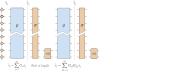
\includegraphics[width=1.\textwidth]{Figs/Sketch/Sketch_circuit.pdf}
		\caption{Sketch. Blue operations applied as an orbital rotation and change the basis of the MPS. Red operations are applied as local gates on the MPS.}
		\label{fig:sketch}
	\end{figure*}

	\emph{Algorithm}: Equipped with the GaMPS representation of the state that allows to span the entire Hilbert space, we present below how to apply a quantum circuit to the GaMPS.
	\begin{itemize}
		\item {\bf Gaussian operations}: Applying a Gaussian unitary $U_{\mathrm{G}}$ to the state is equivalent to update the basis of orbitals as $\tilde{\tilde{\gamma}}_j = \sum_{k=1}^{2L} G_{jk}\tilde{\gamma}_{k}$, as illustrated in Fig.~\ref{fig:sketch}. After each Gaussian operation, we update the orbital frame by successively multiplying the corresponding orthogonal transformations, thereby keeping track of the basis at all times. We dub this basis the instantaneous orbital basis, which defines the space spanned by physical legs in the associated MPS. Each stabilizer and destabilizer becomes non-local superposition of all orbitals. 
		\item {\bf Non-Gaussian operations}: The set of odd majoranas (our \emph{destabilizers}) together with the even ones  forms a complete operator basis, allowing any operator to be expressed as $U = \sum_{i} \phi_{i} s_{u_i}d_{v_i}$. However, the local basis being a superposition of all orbitals, decomposing a gate that is local in a basis different from the stabilized basis (such as the instantaneous one) becomes an all-to-all operation. However, if the gate is $k$-local in some basis, it is possible to build a circuit that extract these $k$ orbitals and makes them the local degrees of freedom of $k$ legs of the MPS. This sequence of operations is depicted in Fig.~\ref{fig:sketch}, where $\sigma$ is the non-local circuit that is applied to the MPS to make the non-Gaussian gate local. For a $2$-local gate, this circuit together with the non-Gaussian gate produce at most an amount $\log(L)$ of entropy.
		\item {\bf Expectation values}: Expectation values are evaluated by decomposing the observable in the instantaneous orbital basis, $\langle \psi | \hat{O} | \psi \rangle = \sum_{k=1}^{L^{r}} a_{k}\langle \nu | \hat{O}_k | \nu \rangle$, where $a_k$ denotes the weight associated with the operator $\hat{O}_{k}$ and $r$ is the number of fermionic modes encoded in the observable. For instance, a density operator $n_\alpha$ can be expanded as $n_\alpha = \sum_{ij} R^{*}_{i\alpha} R_{\alpha j} \hat{\tilde{c}}^{\dagger}_{i}\hat{\tilde{c}}^{}_{j}$, so that $a_{ij} = R^{*}_{i\alpha} R_{\alpha j}$.
	\end{itemize}
	
	\begin{figure*}[t]
		\centering
		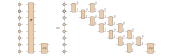
\includegraphics[width=1.\textwidth]{Figs/Sketch/Sketch_permutation.pdf}
		\caption{Sketch of the permutation circuit required for applying a local gate. The circuit $\sigma$ makes the degrees of freedom of the gate that is to apply local in the MPS, and is expressed as a succession of local Givens rotations.}
		\label{fig:permutation}
	\end{figure*}


	\emph{Conclusion and outlook}

	%\textit{Acknowledgement}. The author thank Neil Dowling and Julien Bréhier for discussions. The author was supported by the Deutsche Forschungsgemeinschaft through the cluster of excellence ML4Q (EXC 2004, project-id 390534769) and by the Deutsche Forschungs- gemeinschaft through CRC 1639 NuMeriQS (project-id 511713970).

	\bibliography{Biblio.bib}

      \begin{appendices}
	\end{appendices}


\end{document}

